\chapter{Tools for Design of the Analysis}

For programs with procedure call, context-sensitive analysis is required to improve the precision of data flow facts. It is needed to extend the concurrent analysis technique to inter-procedural level. In the paper, an extension based on the call strings approach was proposed. However we wish to perform inter-procedural analysis using value contexts, for better way to handle recursive programs. \\

A thread now consists of a number of procedure calls, each with their own CFGs. Each thread has an entry procedure with the same name as the thread. Execution of a thread starts with the execution of the start node of the entry procedure. Due to the inter-procedural nature we would need to handle call and return statements by adding edges from the call statement to the root node of the called procedure CFG and edges from the return statement of the called procedure CFG to the statement immediately following the call statement. \\

As an input for the concurrent inter-procedural analysis, we will supply programs with multiple threads with procedure calls in the main thread functions which can be recursive. 

\section{Call Graph Generation}

Call graph construction can be done using Soot\cite{sootguide}. The call graph is available only in whole program mode of soot (-w option). It can be accessed through the \emph{getCallGraph} method. Alternatively, call graph can also be constructed using the VASCO using the class \emph{vasco.callgraph.CallGraphTest} in the \emph{vasco.callgraph package}. VASCO generates a much precise call graph using flow and context sensitive points to analysis over the program. The arguments that need to be given along to run is the classpath containing the soot jar file, the output directory, maximum depth of call chains and the main class indicating the entry point of the program. 

The command is: \newline
\emph{java [-cp CLASSPATH] vasco.callgraph.CallGraphTest [-out DIR] [-k DEPTH] MAIN\_CLASS.} \newline

For example \\
 \emph{java -cp bin:jars/* vasco.callgraph.Test  -out "vasco-output/" -k 9 tests.test} \newline 
 is executed from the project root directory. The class file to be given as input is int the package tests.
 
For the given input program  
\begin{lstlisting}
package tests;
public class test {
	static class A {
		void foo() { bar(); }
		void bar() { }
	}

	public static void main(String[] args) {
		A a1 = new A();
		a1.foo();

		A a2 = new A();
		a2.foo();

		a2.bar();
	}
}
\end{lstlisting} 

We get the calls in the main procedure as \newline
\emph{
	PCG Method : main $\rightarrow$ foo \newline
	PCG Method : main $\rightarrow$ bar \newline
	PCG Method : main $\rightarrow$ foo \newline
	PCG Method : main $\rightarrow$ $<$init$>$ \newline
	PCG Method : main $\rightarrow$ $<$init$>$ \newline
	}

\section{Combined Unit Graph}

We will be using the \emph{CombinedUnitGraph API} to create a sync-CFG required to perform the analysis. This is currently implemented to handle 2 threads and perform intra-procedural analysis. This needs to be improved to handle more than 2 threads and construct inter-procedural CFG as discussed. \\

Creating an intra-procedural CFG :  We first create an object of the \emph{CombinedUnitGraph} class by passing the body of the 1st CFG (for the first thread) to be combined to its constructor. Then, we call the \emph{addLockUnlockUnitsForThread1} 
method to add the lock and unlock nodes in the 1st CFG and store them in respective lists. Now, we
can add the 2nd CFG to this object by calling the \emph{addGraph} method with the 2nd graph
as an argument. This is to be followed by a call to the \emph{addLockUnlockUnitsForThread2} method and finally the \emph{addUnlockToLockEdges} method call in order to complete the construction of the sync-CFG by joining unlock to lock edges for the same lock object. Exact API details are provided in the thesis on Concurrent Analysis of programs.\cite*{btpreport} \\

Consider this input program for intra-procedural live variable analysis:  
\begin{lstlisting}

import java.util.concurrent.locks.Lock;
import java.util.concurrent.locks.ReentrantLock;

public class LiveVariablesInput {
private Lock lock = new ReentrantLock();

private class Thread1 extends Thread {
	public void run() {
		int a=0,b=0;
		lock.lock();
		a = 0;
		lock.unlock();
		
		lock.lock();
		b = a;
		lock.unlock();
	}
}

private class Thread2 extends Thread {
	public void run() {
		int a=0,b=0;
		lock.lock();
		a = 0;
		lock.unlock();
		
		lock.lock();
		a = 0;
		lock.unlock();
	}
}

public static void main(String[] args) {
	LiveVariablesInput ip = new LiveVariablesInput();
	
	Thread t1 = new Thread(ip.new Thread1());
	t1.start();
	
	Thread t2 = new Thread(ip.new Thread2());
	t2.start();
	}
}
\end{lstlisting} 

The combined unit graph creates a sync-CFG in Figure 5.1 for the statements in the jimple representation of the program. The class file is converted to Jimple using Soot.

\begin{figure}
	\centering
	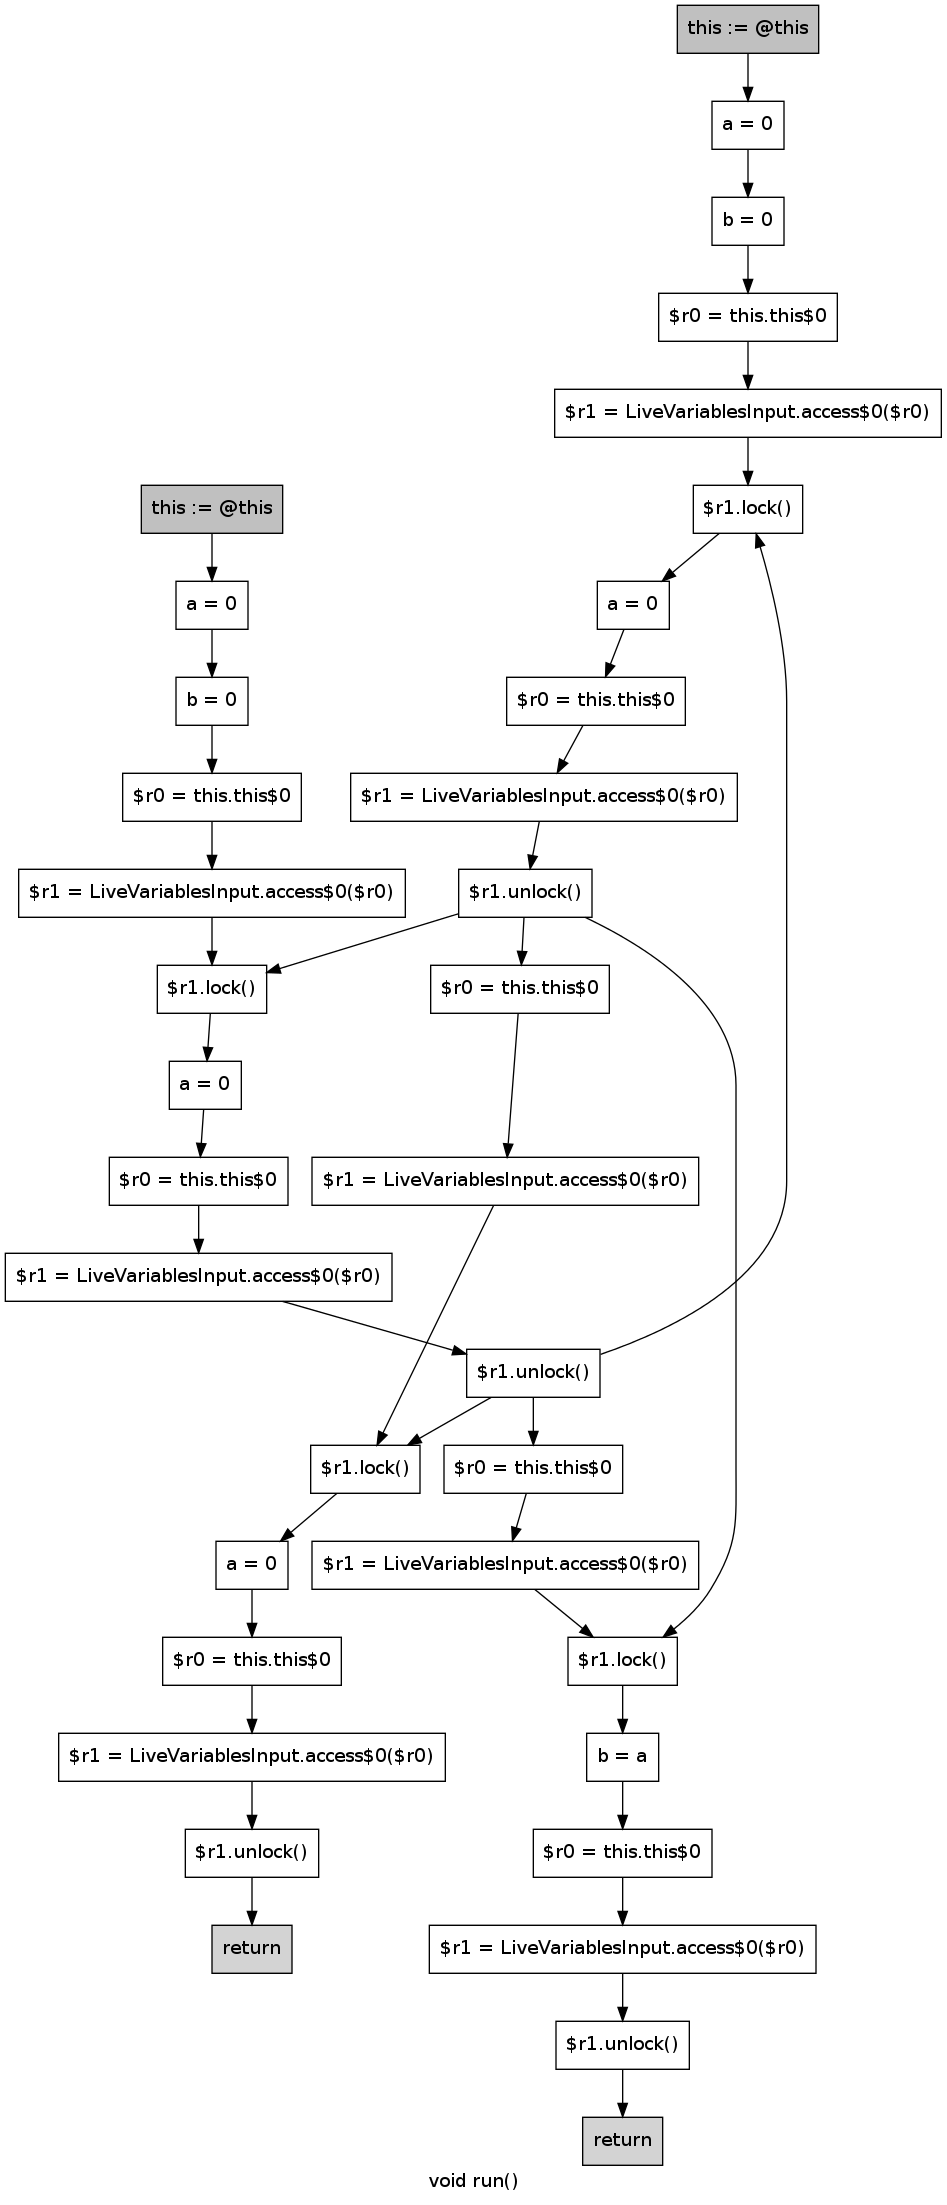
\includegraphics[width=0.6\textwidth]{Figures/combined-cfg.png}
	\caption{Sync-cfg for intra-procedural live variable analysis}
	\label{fig:live var analysis}
\end{figure} 


\section{VASCO framework}

We have already seen the use of VASCO framework to generate precise call graph for inter-procedural programs. VASCO framework is also used to design inter-procedural analysis. To perform and analysis, it is needed to override the methods \emph{normalFlowFunction, callEntryFlowFunction, callExitFlowFunction, callLocalFlowFunction, boundaryValue, copy, meet, topValue, programRepresentation} from the \emph{ForwardInterProceduralAnalysis} (or \emph{BackwardInterProceduralAnalysis} depending on the nature of the analysis).


  



 



